\startchapter{GPU discretization}
\label{chapter:GPUDiscretization}
In the previous chapter we presented an algorithm for fast triangle mesh extraction from \blob scene graphs. The output of that 
algorithm is a list of vertices with their associated attributes such as position, color and normal and a list of triangles that
defines the connectivity of the surface mesh. While the surface mesh is used for rasterization it can also facilitate  
collision detection and contact modeling algorithms as we will see in the following chapters.  In this chapter we propose an improved 
version of that algorithm that can take advantage of the processing capabilities of the GPU and provides real-time \blob rendering performance. 



One of the primary objectives in our modeling framework was to be able to shift from sketching mode into live interactive animation mode
which can enable further enhancements; such as assignment of elastic parameters to the model in an incremental process, e.g. the
modeler can interactively make certain parts of the object stiffer and check out the results by haptically interacting with it or
visually examining the contacts between colliding bodies and with avatar. To make the modelled object amenable to this type of analysis, it has 
to be decomposed into simple shapes called \textit{elements}, which commonly are tetrahedra \cite{Labelle2007}. 
The success of the finite element method depends on the shapes of these tetrahedra, i.e. large dihedral angles cause large interpolation 
and discretization errors and will degrade the accuracy of the numerical simulation, small dihedral angles on the other hand will 
lead to incorrect stiffness matrices associated with the finite element method \cite{Shewchuk}. 


In order to address the tetrahedra extraction stage of the process we propose a GPU accelerated volume tetrahedralization algorithm based on the work of
Labelle \etal \cite{Labelle2007} that produces a smooth tetrahedral mesh. As opposed to their work our algorithm is scalable to number of processors 
available on the graphics processing units and delivers real-time results to support our modeling system.

The contributions in this chapter are as following:

\begin{itemize}
 \item A GPU accelerated polygonization algorithm for rendering complex \blob models. The algorithm scales with the number of stream cores available
 on modern GPU and can be easily extended to support various geometric primitives.
 
 \item A Tetrahedralization algorithm that leverages GPU for high performance volume discretization from \blob models. The output tetrahedral mesh is
 readily available for further physically-based simulations.
\end{itemize}


\section{Related Work}
GPU accelerated rendering techniques has been the topic of interest for the graphics community in the past two decades.
Several GPU-accelerated algorithms have been proposed for fast triangulation and rendering of iso-surfaces that are defined by
volume data-sets, algebraic surfaces and radial-basis functions. In this section we will review the most related works.

Chochl{\'i}k \etal proposed a GPU accelerated polygonization algorithm for dynamically changing implicit surfaces \cite{chochlik2012gpu}. 
Their method is based on the marching tetrahedra (MT) algorithm. The model is partitioned into cubic cells first and then each cell is 
subdivided into 6 tetrahedra to be further processed using the GPU geometry shading stage. The vertices are marked inside if their 
associated field is above zero and outside otherwise. A configuration index is computed per each tetrahedra based on the inside/outside 
vertices. The triangle mesh is produced which is shaded using the fragment shader stage. No further analysis has been made on the performance 
of their algorithm and the input models are limited to time varying simple algebraic surfaces. The used a linear interpolation root finding
method which produces low quality output. 

Buatois \etal proposed a GPU accelerated isosurface extraction method based on MT, similar to Chochl{\'i}k \etal \cite{Buatois2006}. The 
texture memory to transfer the position and field values of the grid vertices. They presented an analysis of the performance of their algorithm
using a fluid simulation volume data-set. They reported that excessive texture fetches can be a bottleneck in the performance of their method.


Tatarchuk \etal proposed a GPU iso-surface extraction algorithm which is a hybrid of marching cubes and marching tetrahedra \cite{Tatarchuk2007}. 
They start by voxelizing an implicit grid into discrete cube cells and then convert that to a tetrahedral representation. They implemented an MT 
algorithm on geometry shader stage of DirectX10 API. For root finding method they fitted a parabola along the intersecting edges and evaluated a 
quadratic equation which produces a better approximation. They tested their system using the visible human volume data-set. Their method
is limited to static volume datasets and is not usable in a data-driven setting where the topology of the underlying model changes. 

With modern hardware and fast GPUs, ray tracing of implicit surfaces is the subject of much research. Knoll \etal \cite{Knoll2009} presented 
CPU and GPU algorithms that can achieve interactive visualization for common algebraic surfaces. The surfaces used in by Knoll \etal are not 
arbitrary implicit models but surfaces generated using traditional kernels or functions. Similar surfaces are presented by Singh and Narayanan
for real-time ray tracing of implicit surfaces using the GPU \cite{singh2010real}. 


Kipfer and Westermann \cite{Kipfer2005} accelerated rendering of implicit surfaces by avoiding redundant computation of edge surface intersections. 
Our method also employs this feature to reduce the overhead. They also use features of the GPU to reformulate the iso-surface identification and reduces 
numerical computations and memory access operations. They used a span-space data-structure to avoid processing non surface intersecting elements.

Kanai \etal \cite{Kanai2006a} proposed a rendering method for sparse low-degree implicit surfaces (SLIM) using ray casting approach. The ray and IS intersection
test has been carried out on the fragment processing stage. They employed level of detail rendering and view frustum culling to speedup the rendering. 
The coefficients for the IS are passed in using textures. They reported high quality and interactive rates for several models. The large number of processed
fragments is the bottleneck in this process and models with lower number of nodes could be rendered slower than more complex models that cover less fragments.
Although Kanai \etal's work is data-driven but the increasing cost of fragment processing is the main bottleneck in their system. Also since they are not
producing any mesh the computations will be lost after rendering.



%Another requirement for the tetrahedral mesh generation is that the triangular surface mesh should be the boundary surface of the tetrahedral mesh. This is needed since 
%after applying the displacements to the volumetric tetrahedral elements the surface vertices should be displaced as well.
\section{Many-cores architectures}
Shrinking of CMOS circuitry has allowed distances between transistors to scale fairly consistently for an extended period of time. The shrinking 
of distances and reduction in size of capacitors allowed hardware architects to clock circuits at a higher rate. This led to Gordon Moore's
famous self-fullfilling prophecy about transistor density and its misinterpretations into the realm of execution frequency and overall performance.

Certainly, increasing frequency allowed the performance of nonparallel code to increase consistently during that time, such that it became an 
expectation for software developers until the early 21st century. During the past decade, it has become obvious the continued scaling of clock 
frequencies of CPUs is not practical, largely due to power and heat dissipation constraints. The reason for this is that power consumption is 
dependent on frequency in a nonlinear manner \cite{gaster2012heterogeneous}. As a second problem, increasing clock frequency on-chip requires 
either increasing off-chip memory bandwidth to provide data fast enough to not stall the linear workload running through the processor or increasing
the amount of caching in the system. 

Due to those reasons the computational hardware available in high-performance workstations shifted from increasingly efficient but complex sequential 
computational units, to smaller units which are not faster than previous generations but the cores are duplicated to be able to execute more threads 
in parallel. This new trend in design can be found in modern CPUs and recent Graphics Processing Units (GPUs). The latest generation of GPUs contains 
hundreds of computation units (4096 in AMD Radeon 7990, 2496 in NVIDIA Tesla K20. For a brief discussion on how to count GPU cores refer to \cite{Fatahalian2008})

This radical architectural change has important consequences on the type of algorithms which are applicable in interactive simulations. In terms of 
programming, general purpose computations on GPUs initially required the use of graphics oriented libraries. The two major GPU vendors released general
programming APIs, CUDA \cite{Nickolls2008} and CTM \cite{peercy2006performance} which provide direct access to the underlying parallel processors of the
GPU, as well as full instruction sets, such as double precision computations and write operations at arbitrary locations. OpenCL which is a multi-vendor
standard was released in 2009, with a programming model very similar to CUDA \cite{gaster2012heterogeneous}. The presented algorithms in this chapter
have been implemented in OpenCL. 

\section{Data Structures}
\label{sec:datastructure}
The \blob linearization step introduced in (section \ref{sec:linearization}) is modified to create a compact representation of the input model in our 
GPU polygonization algorithm. Figure (\ref{fig:datastructure}) depicts this pointerless representation in details.

\begin{figure}[H]
  \centering
  % the following command controls the width of the embedded PS file
  % (relative to the width of the current column)
  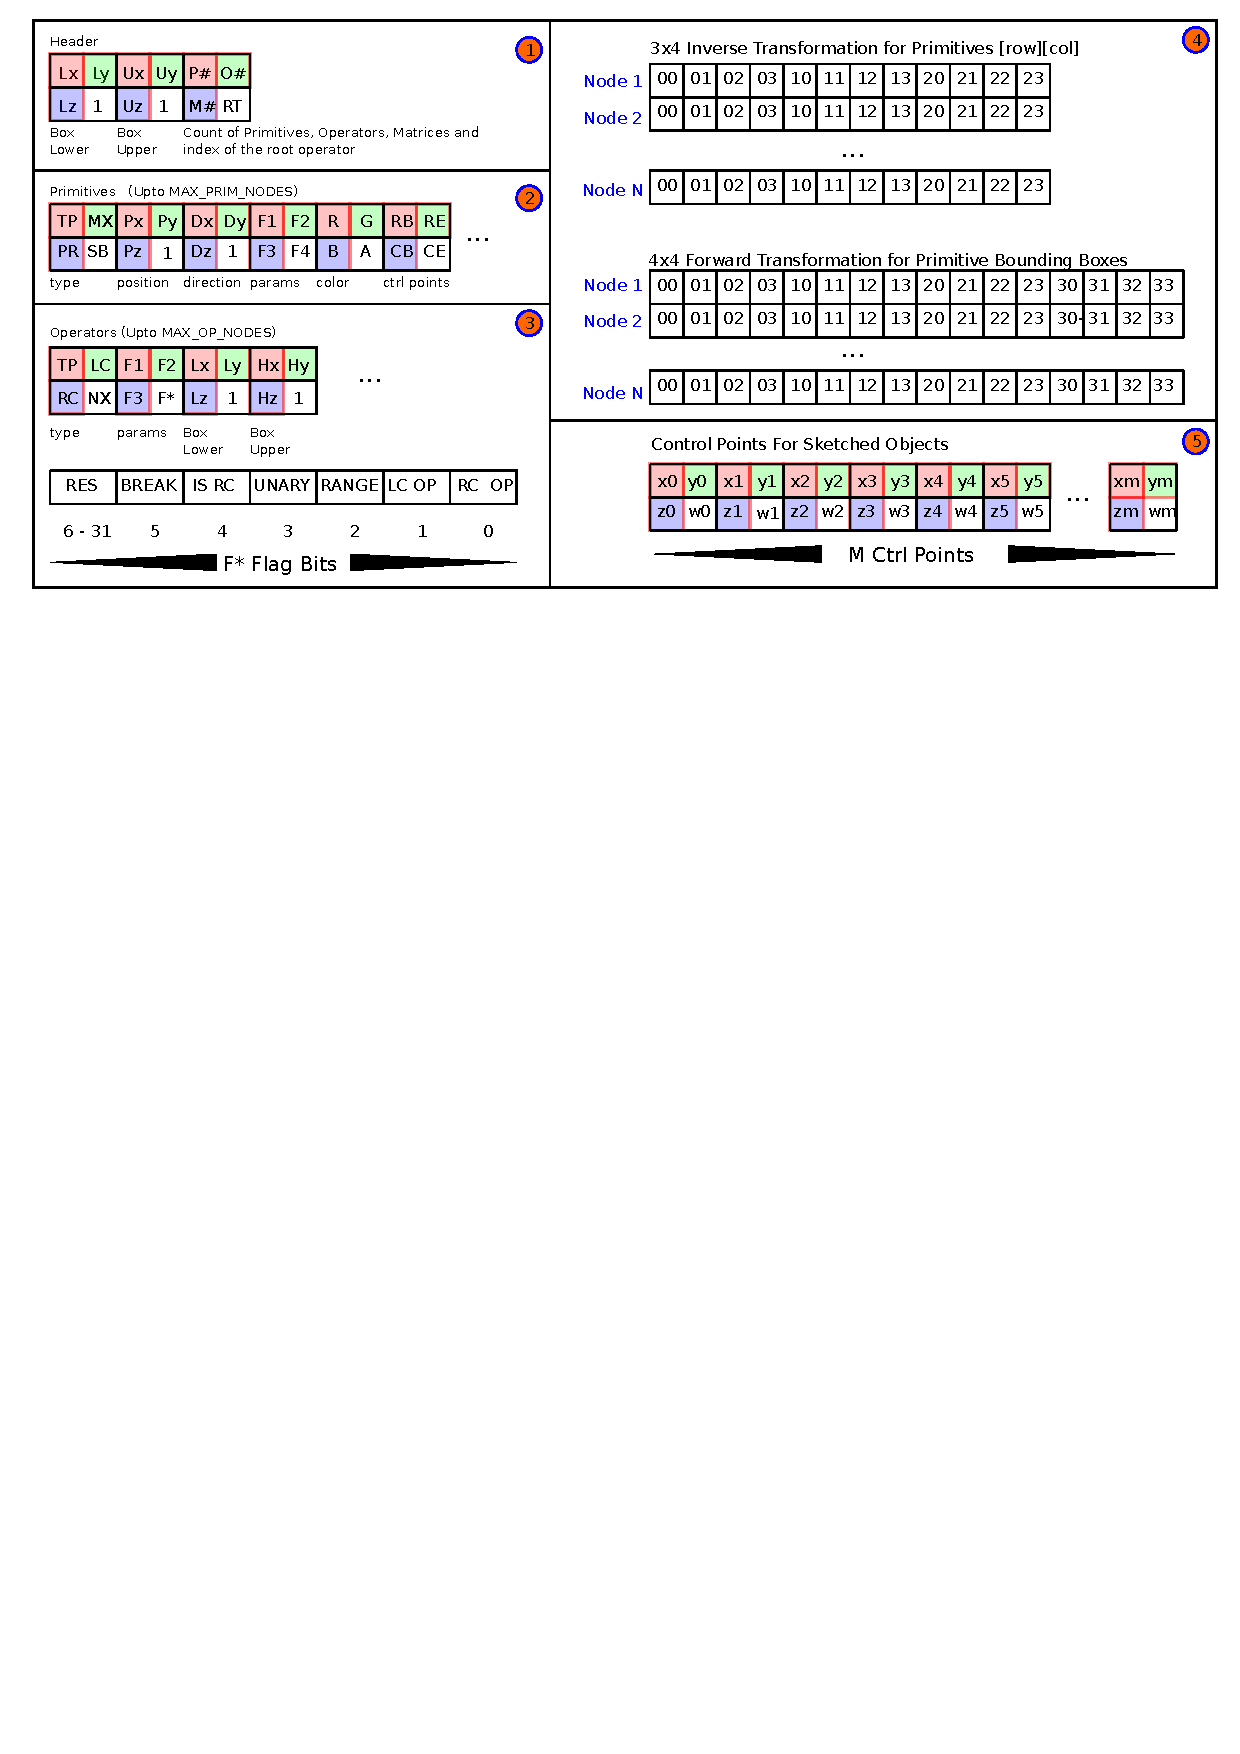
\includegraphics[width=1.0\linewidth]{figures/gpupoly/lineartree.pdf}
  \caption{\label{fig:datastructure}
  {The compact \blob scenegraph representation for GPU polygonization and tetrahedralization algorithms. The structure is aligned at 16 bytes (4 floats). 
  1- The header. 2- Skeletal implicit primitives. 3- Operators. 4- Affine transformation nodes. 5- Control points for sketched objects. Refer to section 
  \ref{sec:datastructure} for details.}
}
\end{figure}

All the structures are aligned at 16 bytes (four floating points) memory addresses (This is similar to the texture accessing techniques in graphical 
shader programming languages such as (GLSL or Cg) where four floats represent the RGBA values of a texel accordingly.) If a primitive node has an associated 
transformation node with a non-identity transformation matrix, that matrix will be stored in the primitive matrices section of the input structure and an associated 
id will be provided to the primitive. The default id is 0 which points to an identity transformation matrix. The inverse of the primitive matrix is 
computed and the first three rows of it will be stored for further field computations. To transform the axis-aligned bounding boxes of the primitives the full forward 
transformation matrix will be stored in the box matrices section of the structure and it can be accessed using the same id provided for the primitive matrix.
Each input data-structure is numbered in figure (\ref{fig:datastructure}) for further reference. We review the details in the following:
\begin{enumerate}
 \item The header section defines the lower and upper corner of the axis-aligned bounding box enclosing the entire model, i.e. the convex hull of the 
 input \blob. The header also contains the count of primitives, operators and transformation nodes. The id associated with the root operator of the 
 tree is also defined in the header.
 \item The primitive section defines the type of skeleton. MX, PR and SB fields are the ids associated with the inverse transformation matrix, the parent and the
 sibling of the node respectively. The following texels define the position, direction, skeleton-specific parameters and the color of the primitive node in 
 that order. For the primitives that are computed from sketched control points (Thin-plate spline \cite{Turk1999, Grasberger} primitives.) the interval of the 
 associated stored control points are provided.

 \item This section defines the operators in the \blob. The type of each operator is the first field defined in the structure. The following fields define the 
 left and right children, in case all the children are primitives and their indices are in a consecutive order (range); LC defines the first child and RC the last child
 included in that closed range of children. The NX field is related to our stackless \blob traversal algorithm which is explained in the following sections and 
 points to the next operator node in the \blob traversal route. The operator-specific parameters and its axis-aligned bounding box are stored next. The F* flag 
 provides more control over the operator and the definition of the bit flags is explained at the bottom of section 3 in the figure. 
 Bits 1 and 0 are set in case the left child or the right child of the current node are operators as well. Bit 2 is set if the LC and RC indices are actually defining 
 a range of skeletal primitives. This situation can happen if a high-level op contains many children such as a global union operator in this case the first two fields
 will be zero as well. If the unary flag is set this operator has only one left child.  Bit 4 is set when the current operator appears as a right node for its parent.
 Bit 5 is the break route flag and is discussed further in our stackless \blob routing algorithm. The rest of the bits are reserved for future use. 
 
 
 \item As mentioned above the inverse of the transformation matrices are computed and the first three rows are stored in our input structure for field computation
 purposes. The elements are depicted in the format of [row][column]. The forward transformation is stored as a 4x4 matrix in a separate input structure for performance
 reasons. 
 
 \item The control points associated with the sketched primitives are all stored in this section. Each control point is defined with their XYZ coordinate and an associated 
 weight. 
\end{enumerate}

\section{Memory foot prints}\label{sec:memory}
In OpenCL and CUDA threads may access data from multiple memory spaces during their execution \cite{Nickolls2008}. Each thread has a private \textit{local} memory. 
OpenCL uses this memory for thread-private variables that do not fit in the thread's registers, as well as for stack frames and register spilling. Each thread block 
has a shared memory visible to all threads of the block that has the same lifetime as the block. Finally, all threads have access to the same \textit{global} memory. 
Programs declare variables in shared and global memory with the \texttt{\_\_local} and \texttt{\_\_global} type qualifier. On a Tesla-architecture GPU, these memory spaces correspond to 
physically separate memories: per-block shared memory is a low-latency on-chip RAM, while global memory resides in the fast DRAM on the graphics board. 

Shared memory is expected to be a low-latency memory near each processor, much like an L1 cache. It can therefore, provide for high-performance communication and
data sharing among the threads of a thread block. Since it has the same lifetime as its corresponding thread block, kernel code will typically initialize data in shared
variables, compute using shared variables, and copy shared memory results to global memory. Thread blocks of sequentially dependent grids communicate via global
memory, using it to read input and write results. 

%Register spilling can increase the number of instructions required to generate prefetch addresses. Ideally only a single instruction would be needed for each prefetch,
% i.e. the prefetch instruction itself. In some cases, as many as 20 extra instructions were added for each prefetch. 
Register spilling occurs whenever the register allocator runs out of registers, and therefore must ``spill'' values by saving and restoring them from memory. Once 
register spilling occurs, the instruction count within a loop body can increase dramatically. 
 
A potential cause of register spilling is the loop unrolling. Once a loop is unrolled, the compiler can optimize across the several replicated copies of the loop 
body. In most cases this allows the compiler to reduce the overall instruction count for the following reasons:
 
 \begin{enumerate}
  \item branch instructions can be eliminated between unrolled iterations
  \item it is more likely that ``hazard'' slots after multi-cycle operations can be filled with independent instructions. 
  \item register allocations can be optimized across the unrolled iterations, possibly eliminating loads and stores.
 \end{enumerate}

On the other hand the potential downside of the loop unrolling is creating too many intermediate values for the register allocator to handle, thus resulting in 
register spilling. One way for the compiler to avoid those register-spilling problems is to perform loop unrolling with a greater awareness of its effect on register 
pressure. 

After analyzing the performance of our OpenCL kernels, register spilling often found to be the major cause for many latencies. Resorting to shared memory spaces, reducing 
number of intermediate variable in field-evaluation kernels and avoiding loop unrolling in some cases helped to optimize the performance. Upon every
change in the input \blob the scenegraph is compacted and transferred from main memory to the GPU. Currently the maximum number of nodes is set at 64K which covers
all of the complex cases we modelled for this thesis. However, for larger \blob models  we can easily increase this amount to support them. The memory footprint of 
our current \blob representation is summarized in table \ref{table:memfootprint}).

\begin{table}[H]
\begin{center}
	 \caption{\label{table:memfootprint}
  {Memory footprint of the input \blob in our GPU polygonization algorithm in bytes. The entire \blob for a model with 64K nodes (primitives and operators) 
  takes about 20MB in our current system.}
}
  \begin{tabular}{ | c | c | c | c | c | c | c | c |}
    \hline    
    Nodes & Header & Primitives & Operators & Prim Mtx & Box Mtx & Ctrl Points & Total \\ \hline \hline
    1 & 48 & 96/Prim & 64/Op & 48/Prim & 64/Prim & 16/Point & 320 \\ \hline
    1K & 48K & 96K & 64K & 48K & 64K & 16K & 320K \\ \hline
    64K & 3072K & 6144K & 4096K & 3072K & 4096K & 1024K & 20M \\ \hline
    1M & 48M & 96M & 64M & 48M & 64M & 16M & 320M \\ 
    \hline
  	\end{tabular}
\end{center}
\end{table}


\section{Stackless \blob traversal}
\label{sec:stackless}
In this section we describe our novel stackless \blob traversal algorithm that completely eliminates the need to maintain a stack during a \blob
traversal and that reduces the number of traversal steps per fieldvalue evaluation. While our multicore algorithm presented in the previous chapter 
benefit moderately from the stackless approach, it improves GPU performance significantly. In high performance rendering algorithms the use of 
hierarchical spatial data structures for acceleration reasons is common. Vising nodes in such structures requires stack-based traversal 
algorithms. Unfortunately, even the latest GPU architectures are poorly suited for implementing such algorithms. 



A complex \blob scenegraph data structure may contain thousands of primitives and operators which can lead to deep tree structures. The fieldvalue 
evaluation process has two stages: ``down traversal'' and an ``up traversal''. During the down traversal stage all operators starting from the root node 
are visited and pushed onto an operators stack until a leaf node (primitive) is reached at which point the field due to the primitive is computed and 
pushed onto a separate fields stack and the next stage which is the up traversal begins. During the up traversal stage the operators are popped out of 
the stack and per each child an associated field is popped from the fields stack for the operator to combine them in its own specific way. The resulting 
field is again pushed back on the fields stack.  This process continues until the operators stack get emptied and the final fieldvalue due to the root node is 
computed and returned.

This naive algorithm requires many push and pop operations which will limit the performance of the traversal process. The other issue relates to the 
inherently dynamic storage requirement for the stack itself. Although, creating a fixed-size stack is possible but since the stack size is a function of
the count of nodes in the input \blob, this will ultimately limit the maximum number of nodes in a complex scene. If $N$ is the maximum number of nodes 
(primitives plus operators) allowed in a \blob model then the minimum number of elements to be stored in the stack during the traversal process 
is given by: $M=\log(N)$ or the depth of the binary tree created by $N$ nodes. Recalling from section \ref{sec:memory} there is very limited amount of
local memory available per each thread executing on the GPU. Keeping the stack in the shared memory will also complicate the implementation and
the access patterns from other threads in the current thread block may impact the performance. Needless to say a stack in global memory will require very expensive 
memory transfers and is not an option for a realtime rendering algorithm. 

Our algorithm is based on the neighbor cell-links concept in the stackless traversal of spatial subdivision trees which is first introduced by Samet \etal 
\cite{Samet1984,Samet1990}. Using a similar technique Popov \etal presented a stackless KD-Tree Traversal for high performance GPU ray tracing algorithm \cite{Popov2007}.

\begin{figure}[H]
  \centering
  % the following command controls the width of the embedded PS file
  % (relative to the width of the current column)
  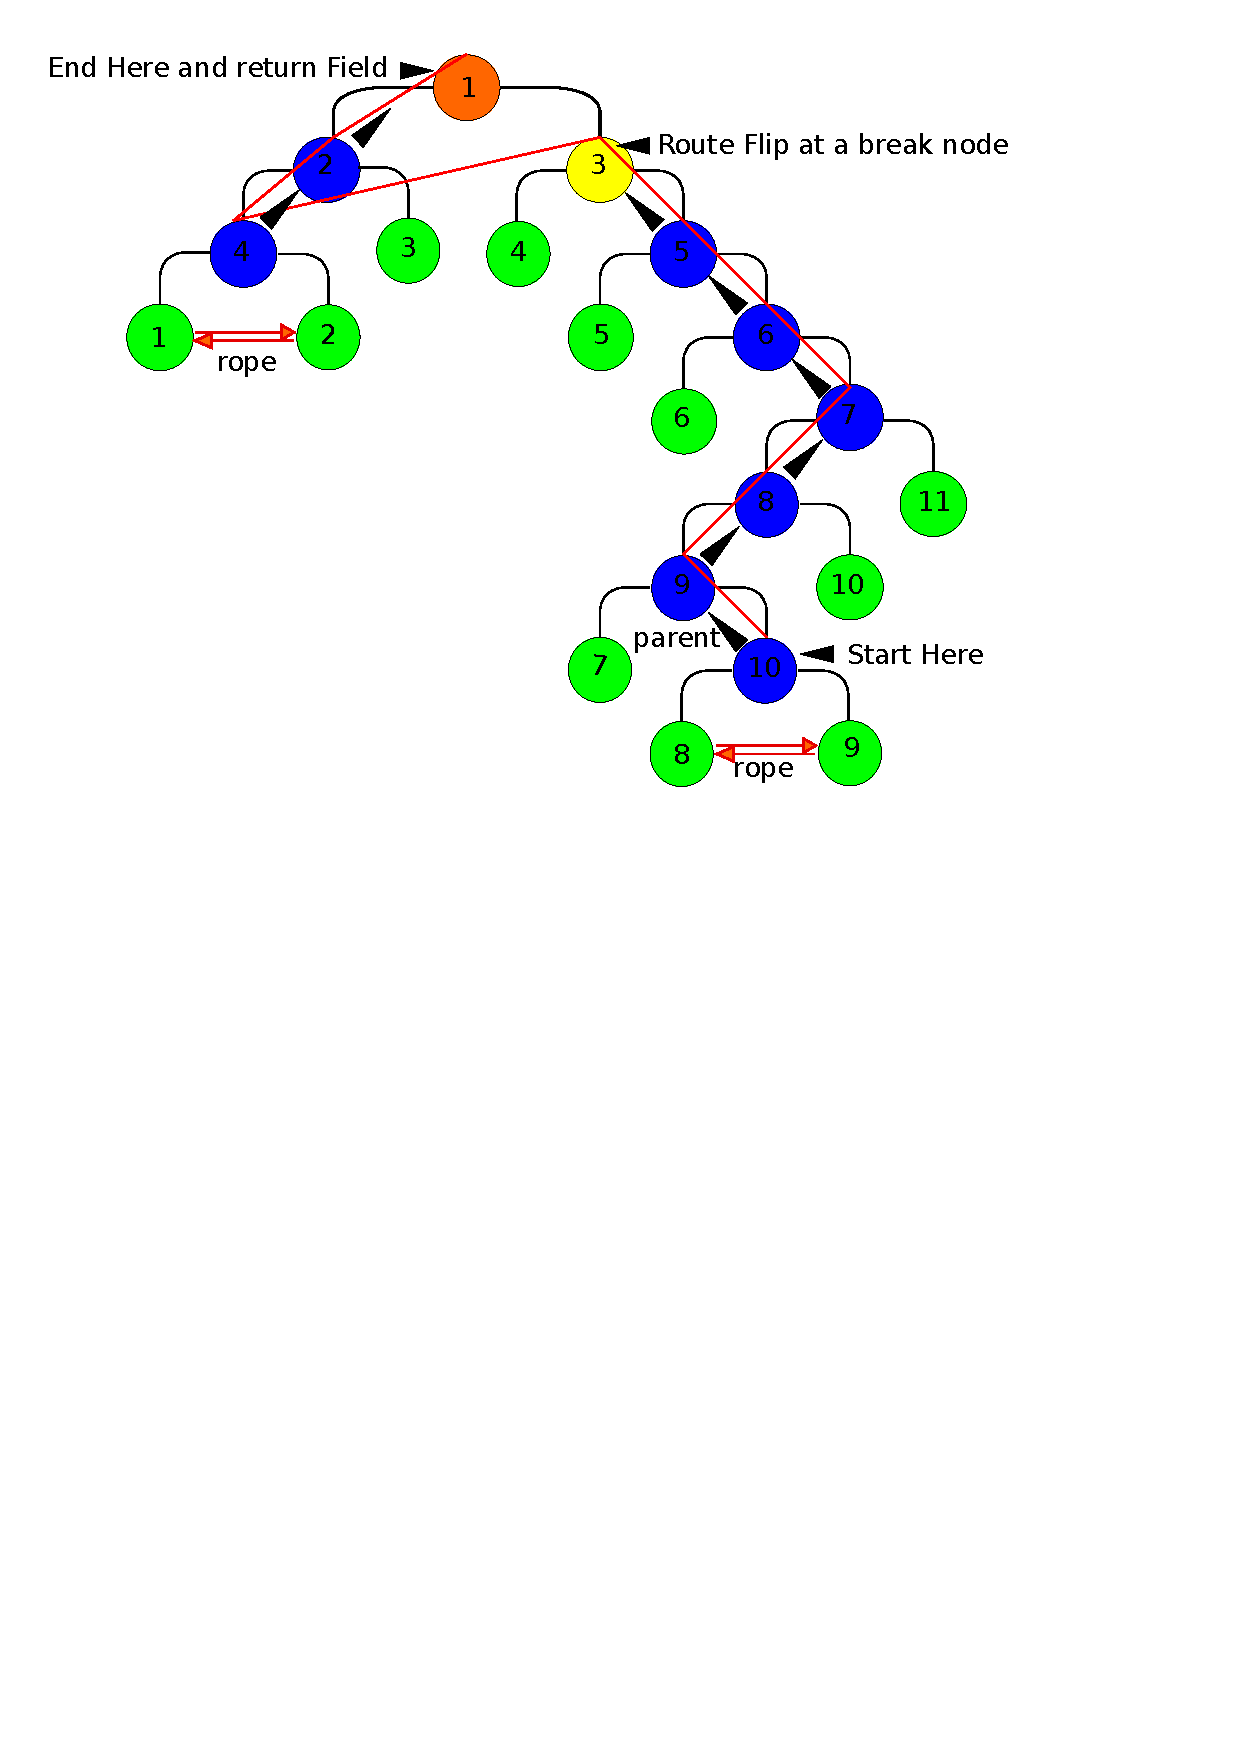
\includegraphics[width=1.0\linewidth]{figures/gpupoly/stackless.pdf}
  \caption{\label{fig:stackless}
  {Stackless \blob traversal algorithm performs faster on deep tree traversals. The route is computed once and encoded into the tree upon transferring the input 
  data structures to the GPU.}
}
\end{figure}

We start by computing a route to visit all nodes in the \blob. This process is done once and is not a bottleneck in the system.
Using the naive \blob traversal algorithm the nodes are visited from root to leaves. Two stacks are used in this process, an
operators stack $S1$ and a \text{break} nodes stack $S2$. The latter is defined in the following:

\begin{enumerate}
 \item If one of the children is an operator and the other is a primitive. Let $A$ be the name of that child operator. The parent for $A$ is set 
 to the current node and then it is pushed onto $S1$.
 
 \item If both children are operators. The right child is set as a \textit{break} node (The route at break nodes will be flipped to 
 the left branch of the tree, see figure \ref{fig:stackless}) then it is pushed on to $S2$.
 
 \item If the two children are both primitives: First the root of the \blob is set to the current node if it hasn't been set before.
  (Refer to the \blob header format in figure \ref{fig:datastructure} for the location of the root field $RT$) 
  A rope is created between the two primitives, linking the two nodes and a break node $B$ is popped from $S2$. 
  The next node for $B$ is set to the current node.
 
  
 \item The process is continued until $S1$ is emptied.
\end{enumerate}


Figure \ref{fig:stackless}, shows the final route for a sample \blob. The benefits of this type of routing encoded into the tree
is that there is no need for storing a deep stack for tree traversals. The kernel functions written in OpenCL to compute the field
has the following prototypes. The structure of the input blobtree are as following:
arrHeader4: Defines the header of the linear blobtree.
arrOps4: The operators structure for the compact blobtree.
arrPrims4: The compact structure for the primitives.
arrMtxNodes4: The input transformation matrices associated with primitives.


\begin{lstlisting}[frame=single]
//Computes the field at point v due to a skeletal primitive. 
float PrimitiveField(unsigned int idxPrimitive, float4 v,			
		     __global float4* arrOps4,
		     __global float4* arrPrims4, 
		     __global float4* arrMtxNodes4);

//Computes the field at point v due to an operator.
float OpField(unsigned int idxPrimitive, float4 v,			
	      __global float4* arrOps4,
	      __global float4* arrPrims4, 
              __global float4* arrMtxNodes4);

/*A Range is an operator with all primitive children. Left child field 
in this operator defines the index of the first primitive child and 
right child is the index of the last primitive.*/
float RangeField(float4 v, unsigned int idxOp, 						
		 __global float4* arrOps4,
		 __global float4* arrPrims4, 
		 __global float4* arrMtxNodes4);

/*The field due to a branch of the tree until a break node is reached. 
lf and rf are the fields previously computed for the left and right branches 
of the tree (initially zero)*/
float BranchField(unsigned int idxBranchOp, unsigned int* lpNextOp, 
		  bool* lpIsBreakOp, float4 v, 
		  float lf, float rf,
		  __global float4* arrHeader4,
		  __global float4* arrOps4,
		  __global float4* arrPrims4, 
		  __global float4* arrMtxNodes4);
		  
/*The main field evaluation function which will call the other four functions accordingly.*/
float Field(float4 v,			
	    __global float4* arrHeader4,
            __global float4* arrOps4,
	    __global float4* arrPrims4, 
	    __global float4* arrMtxNodes4);
\end{lstlisting}


\section{GPU Surface Extraction Algorithm}
In this section we present our GPU polygonization algorithm which is based on our novel field value evaluation technique described
in the previous section. Since the following steps are implemented using OpenCL on the GPU we will use the term \textit{kernel} which 
refers to the single thread of execution on the GPU. Please refer to section \ref{sec:memory} for a description of the memory model for
general purpose GPU (\textit{GPGPU}) programming.

We start by computing the axis-aligned bounding box of the model by traversing the tree from root to leaves 
and applying the transformation matrices at leaf nodes (primitives). Using the \textit{cellsize} parameter supplied by the user the 
bounding box is divided into a grid of voxels. The kernel function \textit{ComputeAllFields} will compute a fieldvalue per each
vertex of this voxel grid and store that value in the format of \textit{XYZF} where \text{XYZ} denotes the vertex position and 
\textit{F} is the so-called field at that position. 


After computing all the fields, the grid edges are processed in the following order. 
Each vertex in the grid can be connected to upto 6 other adjacent vertices. Starting from the lower corner of the voxel grid 
the kernel function \textit{ProcessEdges} visits the corresponding vertex in the grid and examines only the edges that start 
from that vertex and connect to the adjacent vertices in the next index step. This way all edges in the voxel grid are checked 
and redudant traversals can be avoided. Needless to say that at boundary vertices it may process less than 3 edges per each 
vertex (i.e. the ones that are within the convex-hull of the model). Upon each kernel run at this stage the index address to 
the corresponding vertex and it 3 other adjacent vertices is computed as shown in the algorithm \ref{alg:processedgeskernel}. Per each vertex
an inclusion query is performed (i.e. The fieldvalue at that vertex is compared against the isovalue. If it is greater than or equal 
the isovalue the vertex is considered inside otherwise outside the model). Two values are stored before completion of this kernel call. 
The first is the count of crossed edges at that vertex and the second one is a 3 bits flag which basically locates the intersected 
edges along x, y or z axes.


\begin{algorithm}[H]
\caption{\textit{ProcessEdges} kernel function counts the number of intersected edges and their corresponding axes. This kernel runs per each
vertex of the voxel grid.}
\label{alg:processedgeskernel}
\begin{algorithmic}[1]	
  \STATE $v = queryVertexInclusion(i, j, k)$
  \STATE $vx = queryVertexInclusion(i+1, j, k)$
  \STATE $vy = queryVertexInclusion(i, j+1, k)$
  \STATE $vz = queryVertexInclusion(i, j, k+1)$
  \STATE $count = (v \xor vx) + (v \xor vy) + (v \xor vz)$
  \STATE $flag = (((v \xor vx) << 2) or ((v \xor vy) << 1) or (v \xor vz))$
\end{algorithmic}
\end{algorithm}


After processing all edges with the kernel given in listing \ref{alg:processedgeskernel}, the \textit{EdgeBuffer} 
contains the count of intersected edges per each vertex in the voxel grid. In order to compute the total number of 
output vertices in the triangle mesh the prefix-sum (\cite{Sengupta2007}) of \textit{EdgeBuffer} is computed and
stored in a separate gpu memory buffer called \textit{ScannedEdges}. The total number of vertices is the sum of the
last element in both the \textit{EdgeBuffer} and \text{ScannedEdges}. Before computing the vertex 
attributes (position, color and normal) the GPU memory buffers are allocated on the device global memory using the total number 
of vertices computed in the previous step. 

After this stage the vertex attributes of the mesh can be computed by executing a root finding method on the intersected 
edges and storing the output vertices in their appropriate buffer locations using the offsets in \textit{ScannedEdges}.
We used a Newton-Raphson root finding method which converges to the iso-surface using the gradient of the field \cite{Matthews1987}.
At each iteration the root is displaced closer to the surface according to the method given by Overveld \etal (\cite{VanOverveld2004}):

\begin{equation}
 r = r + \frac{\left(iso - f(r)\right)}{\nabla V(r).\nabla V(r)}
\end{equation}

Where $r$ is the root, $f(r)$ is the field at $r$ and $\nabla V(r)$ is the gradient of the field at $r$.
A maximum iterations of 4 is sufficient to provide smooth results in our tests. 
After computing the root position other attributes such as the color and normal at that vertex are also computed and stored in their 
designated buffers. The next step is to process the cells in the voxel grid in parallel and compute a configuration index per each cell
for extracting the topology of the triangles. There is no \blob traversal at this stage since the computed fields will be provided
to the kernel function. The configuration table is passed in as a texture image and being accessed using texture sampler for 
fast access. The number of triangles that are output per each cell is stored in a buffer called \textit{FaceBuffer}.

In order to find the total number of triangle elements a prefix-sum scan is applied to the \textit{FaceBuffer} array 
in the same way that total number of vertices is computed previously. The buffer \textit{ScannedFaces} will be used to hold the 
offset values per each cell. 

The final stage in our GPU polygonizer is producing the triangles. For this purpose the kernel function \textit{GenerateFaces} 
is called per each cell in the voxel grid. No \blob traversal is required for this stage. Only the cells which intersect with the 
iso-surface will be further processed. Upon each kernel run the indices for the eight vertices of the current cell is computed. 

To process cell configurations we used the improved marching cubes table by Dietrich \etal 
\cite{Dietrich2009}, which avoids most of the small and badly shaped triangles. The table is supplied to the kernel as 
a texture of size 256 rows by 16 columns. To access the entries in the table the texture sampler on the hardware 
can be used. Per each cell the configuration index is computed using the previously stored fields. Each entry in the table is the 
index of an edge in the cell (There are 12 edges per each cell). Algorithm \ref{alg:generatefaceskernel} shows how the 
triangle elements are computed at this stage.

\begin{algorithm}[H]
\caption{\textit{GenerateFaces} kernel function computes the triangle indices per each cell and outputs them directly into an
OpenGL index buffer for rasterization. All the buffers can be read back later from the GPU and stored.}
\label{alg:generatefaceskernel}
\begin{algorithmic}[1]	 
  \STATE $index = globalCellIndex(i, j, k, dim)$
  \STATE $config = cellconfig(i, j, k)$
  	  \IF{$config == 0$ or $config == 255 $}
	  \STATE return;
	  \ENDIF	
   \STATE $cellcorners = cellCornerIndices(i, j, k, dim)$
   \STATE $offset = ScannedFaces[index]$
   \STATE $count = FaceBuffer[index]$
   \FOR{$i=1 \to $count}
	 \STATE $edge = sample($configtable$, int2(edge, index))$
	 \STATE $start = EdgeStartIndex[edge]$
	 \STATE $axis = EdgeAxis[edge]$
	 \STATE $elements[offset + i] = ScannedEdges[cellcorners[start]] + axis$
   \ENDFOR				

\end{algorithmic}
\end{algorithm}


Each cell may contribute up to 5 triangles. Line 11 and 12 in algorithm \ref{alg:generatefaceskernel} 
assigns the start index of an edge and its associated axis using two constant buffers supplied to the kernel for this purpose. 
The element entry is computed as an index to the global vertex buffer. The \textit{ScannedEdges} 
buffer holds the global offset for all the intersected edges as discussed previously. 

\section{Analysis and Results}
In this section we review the effects of the previous optimizations on the overall performance of the system.
In our experiments we tested the effect of the stackless \blob traversal algorithm using a set of models created 
with our incremental modeling system. To make a fair comparison the same algorithm implemented on the GPU using
the OpenCL framework once with the stack and the other time with the stackless method presented in section 
\ref{sec:stackless}. The results are shown in the following table:



\begin{table}[H]
\begin{center}
	 \caption{\label{table:stackless}
  {Stackless \blob traversal improved the performance of our \blob traversal significantly.
  Here is the comparison of fieldvalue evaluation on the GPU comparing stackless approach to a stack-based implementation for 
  some models. Timings are average of 100 runs.}
}
  \begin{tabular}{ | c | c | c | c | c | c |}
    \hline    
    Model Name & Field Queries & Grid & Stack-based (ms) & Stack-less (ms) & Speedup \\ \hline \hline
    Tumor & 16240 & 29*20*28 & 21 & 0.8 & 26x\\ \hline
    cake & 18975 & 33*23*25 & 17 & 1 & 17x\\ \hline
    3slabs & 28750 & 46*25*25 & 30 & 2 & 15x \\ \hline
    \hline
  \end{tabular}
\end{center}
\end{table}


\begin{figure}[H]
  \centering
  % the following command controls the width of the embedded PS file
  % (relative to the width of the current column)
  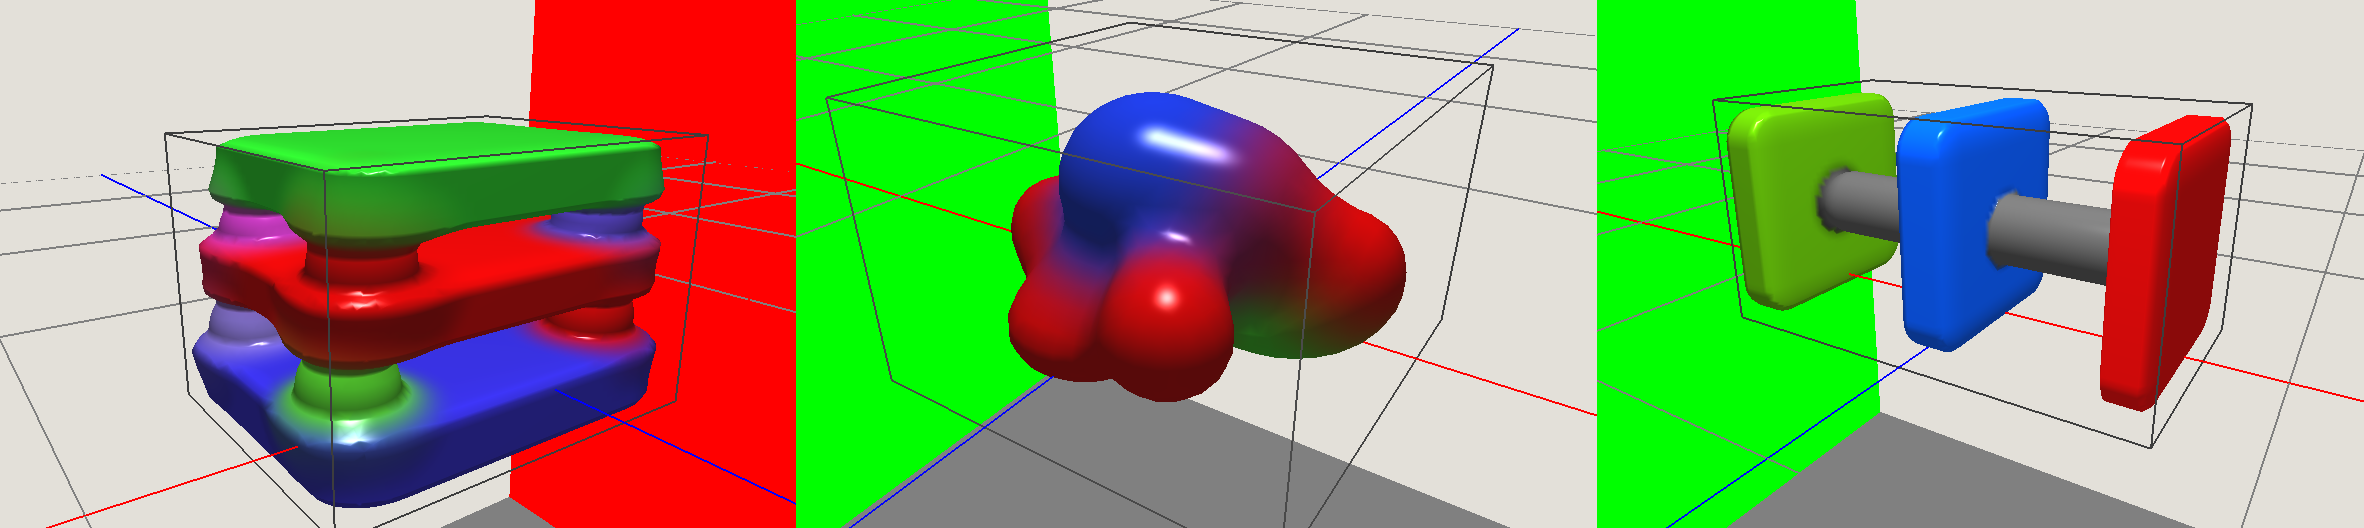
\includegraphics[width=1.0\linewidth]{figures/gpupoly/combined_models.png}
  \caption{\label{fig:combinedmodels}
  {Sample models for testing our GPU polygonization method. From left to right: Cake, tumor and 3slabs.}
}
\end{figure}

When using stacks, the register spilling phenomenon mentioned previously will degrade the performance due to the higher cost of accessing 
shared memory. Conditional push and pops in stack-based method also stalls the performance of the kernels.  

Faster field evaluations using the stackless algorithm also improved the performance of our root-finding method and the overall
polygonization time. In the following we review per kernel time break-time which provides a close look at hotspots (most time-consuming 
locations) in our implementation. 

%Tumor: Fields: 2, Edge: 1, EdgeBufferScan: 22, Vertex: 44, Cell: 1, FaceBufferScan: 18, Faces: 17, Total: 105
%Cake: Fields: 1, Edge: 1, EdgeBufferScan: 19, Vertex: 58, Cell: 2, FaceBufferScan: 17, Faces: 10, Total: 108
%3Slabs: Fields: 1, Edge: 1, EdgeBufferScan: 18, Vertex: 40, Cell: 1, FaceBufferScan: 17, Faces: 1, Total: 79

\begin{figure}[H]
  \centering
  % the following command controls the width of the embedded PS file
  % (relative to the width of the current column)
  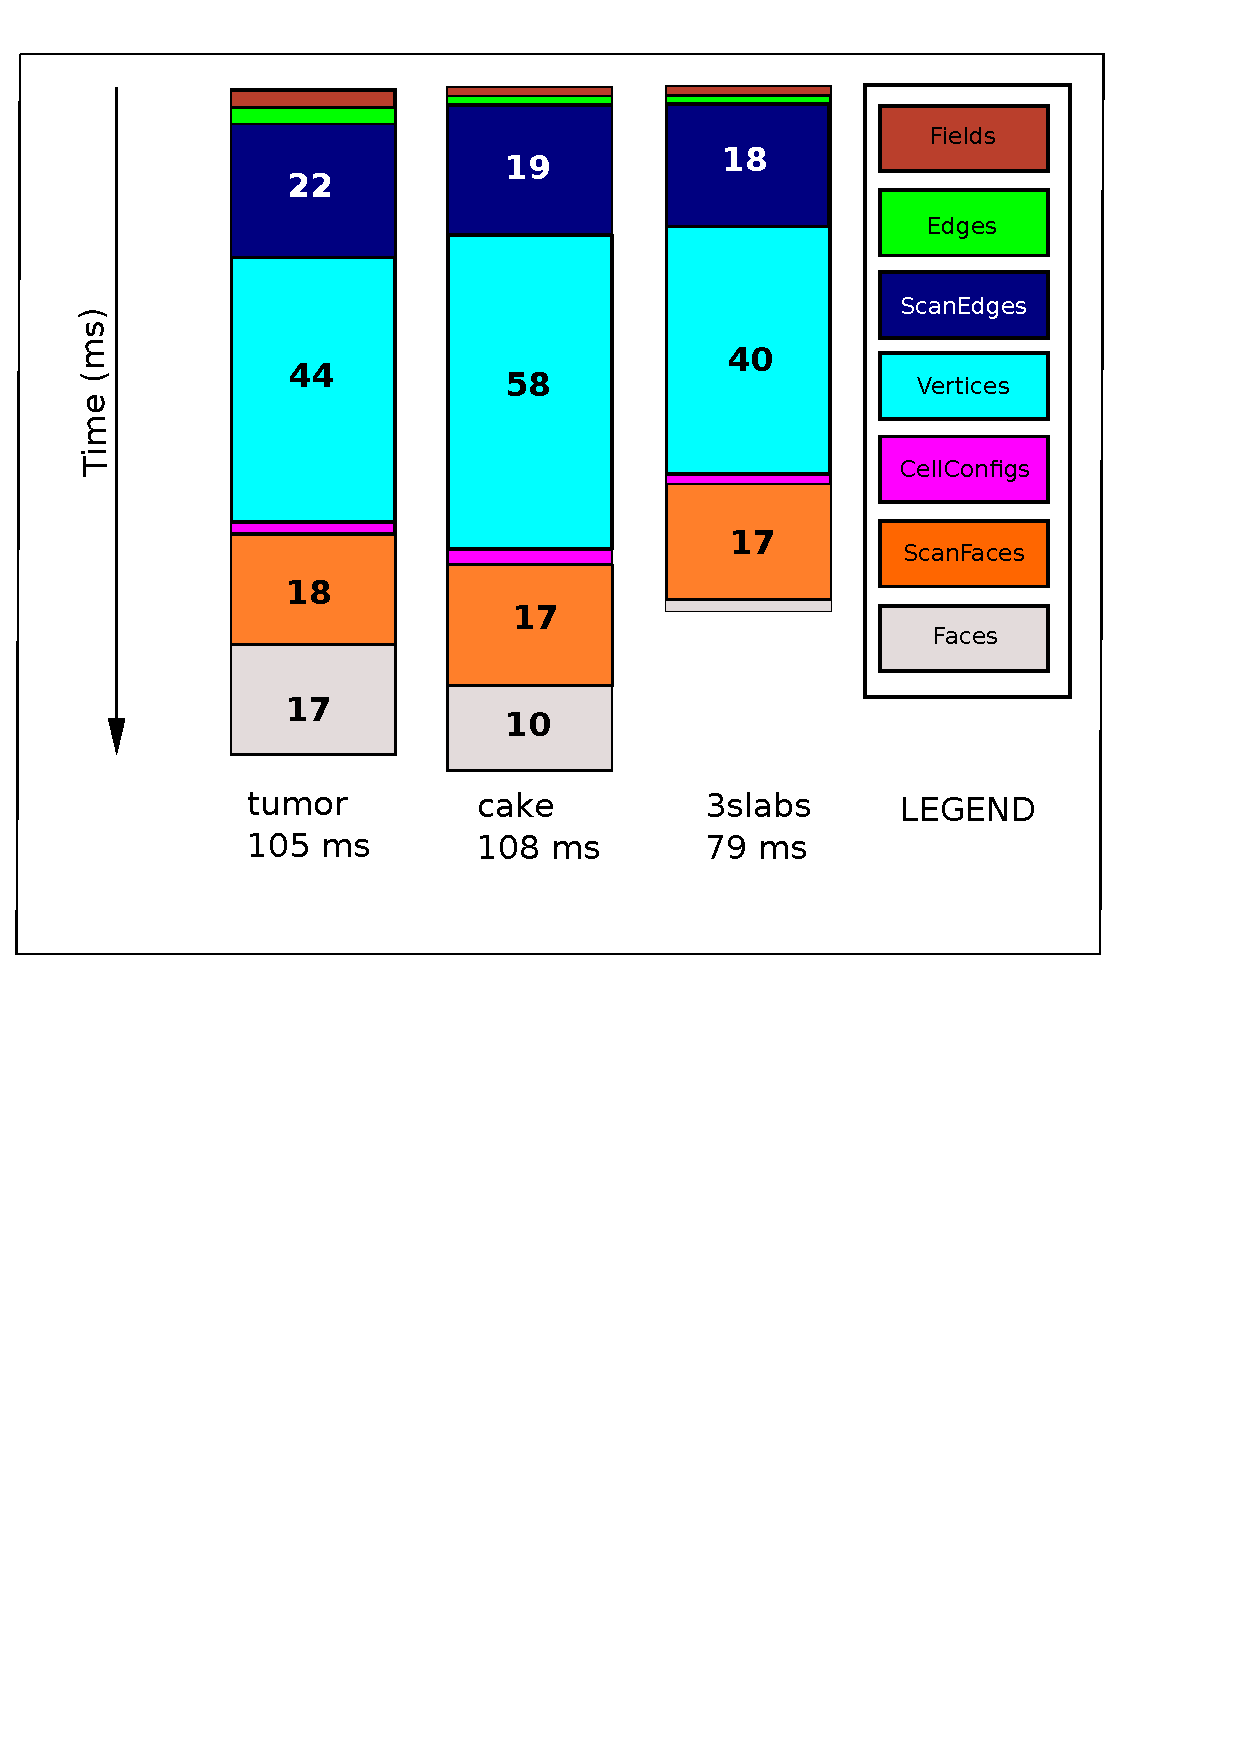
\includegraphics[width=1.0\linewidth]{figures/gpupoly/breakdownpoly.pdf}
  \caption{\label{fig:breakdownpoly}
  {Polygonization time breakdown in milliseconds for the three models shown in the previous section. Vertex processing is the most compute-intensive
  stage due to the Newthon-Raphson root finding method employed and the evaluation of colors and normals which require additional traversals.
  }
}
\end{figure}

As it can be seen computing vertices is still the most time-consuming stage due to the extra tree traversals required for high quality 
gradiant-based Newthon-Raphson method for root-finding. Computing other attributes such as colors and normals would also need 1 and 4 
traversals respectively. The prefix-sum scan operator employed here uses multi-pass computing. The extra cost of kernel invokations
increased the cost of using these operators. Several optimizations can be performed to benefit the overall performance. By 
vectorizing all kernels the core SIMD units can be used more efficiently. 
In Nvidia and AMD GPUs the local memory is divided into memory banks. Each bank can only address one dataset at a time, so if a halfwarp (16 threads)
tries to load/store data from/to the same bank the access has to be serialized (this is called a bank conflict). 
For NVidia GT200 GPUs there are 16 banks and in Fermi card this number is 32. If each thread in a halfwarp accesses successive 32bit values
there are no bank conflicts. An exception from this rule are broadcasts: If all threads access the same address, the value is only read once and
broadcasted to all threads (e.g. For GT200 it has to be all threads in the halfwarp accessing the same address).

The prefix-sum scan operator can also be implemented in such a way that the memory-bank conflicts be avoided and the data-access
be performed in parallel.


\section{GPU Tetrahedralization}


















